
\clearpage

\section{GEANT4}
\label{sec:GEANT4}
GEANT4(\textbf{GE}ometry \textbf{AN}d \textbf{T}racking - \textbf{4} versión) es una plataforma computacional para la simulación de diversos procesos físicos que se centra en la interacción de partículas viajando a través de la materia haciendo uso de Montecarlo. Geant es creado en 1974 por el CERN pensado originalmente para la simulación de experimentos en física de altas energías, esto cambiaría con el desarrollo de subsecuentes versiones las cuales serían empleadas en muchos otros campos, su cuarta versión Geant4 es publicada en 1998, esta última a su vez también ha tenido diversas versiones actualizadas cada año, su lanzamiento más reciente ha sido Geant4-10.5.p01 y su versión beta Geant4-10.6-beta ambas versiones liberadas en el presente año,  cuenta  con áreas de aplicación que incluyen física de altas energías, física espacial, física médica, transferencia tecnológica, entre otras, su desarrollo, aplicación y mantenimiento son debido al equipo colaborativo a nivel global Geant4 Colaboration los cuales se centran en que el software pueda ser lo mejor posible.
\\
\\
GEANT4 se proporciona bajo la licencia \href{https://geant4.web.cern.ch/license/LICENSE.html}{\color{blue}{Geant4 Software License}}.

\subsection{PDB4DNA}

PPB4DNA es una aplicación relativamente nueva de Geant4 creada por Geant4-DNA project, se basa en el uso adicional de una librería construida en c++ llamada PDBlib, la cual permite hacer uso de la estructura atómica de una molécula de ADN al extraer datos que se encuentran en un archivo .pdb para posteriormente ser usados en Geant4 para evaluar el daño inducido por partículas ionizantes al mismo, mediante un conteo de rompimientos simples, rompimientos dobles y su correspondiente deposición de energía.

El objetivo principal de Geant4-DNA project es extender Geant4 con diversos procesos para el modelar el daño biológico inducido por radiación ionizante en la escala del ADN, es coordinado desde el 2008 por el National Institute for Nuclear and Particle Physics (IN2P3) del National Centre for Scientific Research (CNRS) en Francia.


\subsubsection{PDB}
Un archivo .pdb (Protein Data Bank) es un archivo de texto que contiene la información estructural de una molécula, se compone de cientos a miles de líneas y en general debe contener lo siguiente\\
HEADER: Registra si la molécula es ADN o proteína.\\
REMARK: Designa comentarios los cuales pueden dar información relevante.\\
ATOM: Registra el símbolo del átomo, id de cadena, numero de residuo o nucleótido y coordenadas espaciales x y z. \\
Para observar un ejemplo de cómo está conformado un archivo pdb véase figura ~\ref{fig:pdbesq}.
\begin{figure}[htbp]
    \centering
    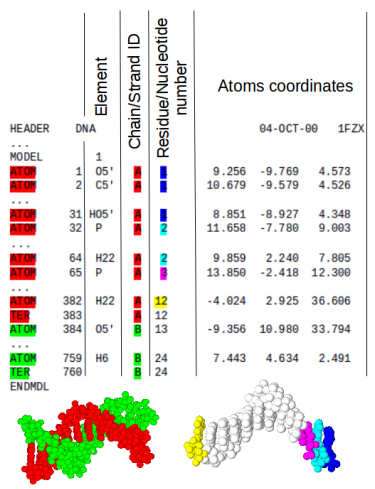
\includegraphics[width=.5\linewidth]{./Figures/pdb.png}
    \caption[Esquema de un PDB]{Esquema de un PDB, imagen tomada de\cite{pdblib}} % se puede realizar grafico en vmd}
    \label{fig:pdbesq}
\end{figure}

\subsubsection{pdb reader}
Está funcionalidad presente en PDBlib permite leer la estructura molecular de un pdb en Geant4 sin la necesidad de usar otras librerías de terceros, la función se encarga de recolectar la siguiente información: elemento, id de cadena, numero de residuo y coordenadas del átomo, mediante el uso de palabras clave como ATOM y TER\cite{pdblib}.
\subsubsection{Visualización}
Pdb4dna viene preestablecido con la molécula 1ZBB esto debido a que describe la estructura de ADN más grande que se encuentre en formato pdb, el ejemplo hace uso de la geometría de Geant4 simplemente para objetivos de visualización como formas, distribución espacial, materiales y atributos de visualización para cada átomo, por ahora PDB4DNA solo presenta tres modos de visualización, esferas ligadas(baricentros), vista atómica (VDW) y residuos\cite{pdblib}.

\begin{figure}[htbp]
    \centering
    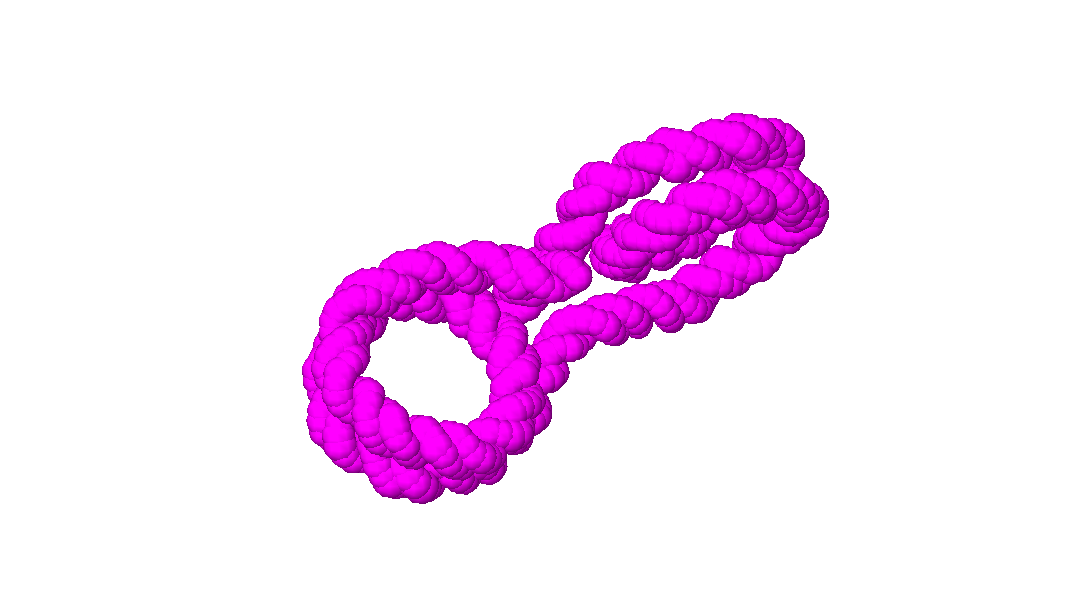
\includegraphics[width=.7\linewidth]{./Figures/ba.png}
    \caption{Barycentros}
    \label{fig:ba}
\end{figure}


\begin{figure}[htbp]
    \centering
    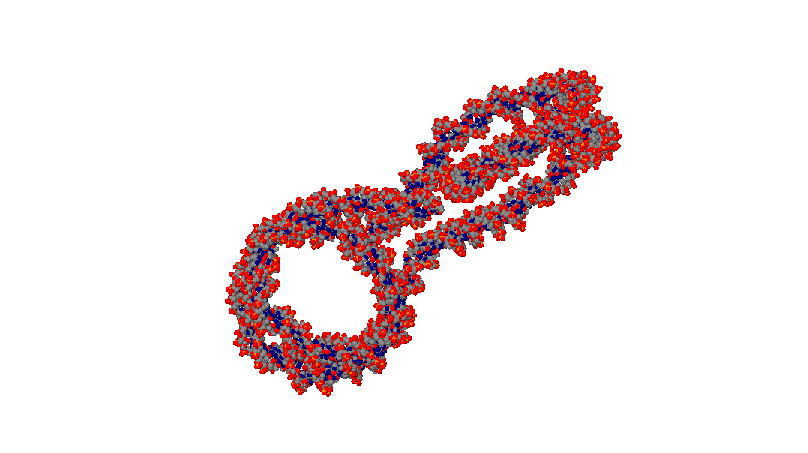
\includegraphics[width=.7\linewidth]{./Figures/cpk.png}
    \caption{VDW}
    \label{fig:cpk}
\end{figure}

\begin{figure}[htbp]
    \centering
    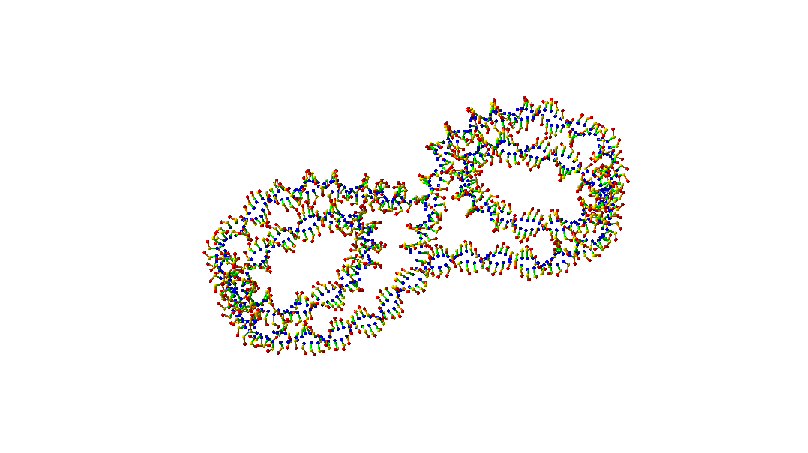
\includegraphics[width=.7\linewidth]{./Figures/re.png}
    \caption{Residuos}
    \label{fig:re}
\end{figure}

\subsubsection{Simulación}
Debido a que Geant4 no contiene secciones transversales definidas para ADN, las simulaciones son realizadas en agua y las deposiciones de energía resultantes son entonces alocadas en grupos de átomos constituyendo la molécula de ADN, para este propósito se hace uso de un bounding box(caja delimitadora) el cual es un volumen constituido de agua con dimensiones correspondientes a la respectiva molécula de ADN, la lista de física empleada es Geant4-DNA adaptada a micro y nano dosimetría, los procesos de esta extienden la física para electrones, hidrógeno, átomos de helio y algunos iones\cite{pdblib}.

\subsubsection{Algoritmo para encontrar el átomo más cercano}
Es necesario el uso de un algoritmo cuyo objetivo de este es alocar la deposición de energía en un elemento (azúcar base o fosfato) del nucleótido para luego deducir rompimientos de cadena simples y rompimientos dobles.
Para empezar se forman múltiples esferas a partir del baricentro geométrico de cada nucleótido, el radio de cada esfera es la máxima distancia entre el baricentro y las coordenadas de los átomos que constituyen el nucleótido, incluyendo el máximo radio de Van der Waals (1.8 Angstrom para el elemento del fósforo), si una deposición de energía es localizada en una esfera ligada un segundo proceso verifica los radios de Van der Waals, para encontrar el átomo del nucleótido más cercano a dicha deposición. debido a que las esferas ligadas de los nucleótidos se superponen, los dos nucleótidos más cercanos son incluidos en el algoritmo, cuando se cumple un evento, el algoritmo retorna la deposición de energía, la cadena de ADN, el id de nucleótido, y el id del grupo sea base, fosfato o azúcar, todo este proceso puede verse con más claridad en las figuras ~\ref{fig:deepbox} y ~\ref{fig:algoritmo}.


\begin{figure}[htbp]
    \centering
    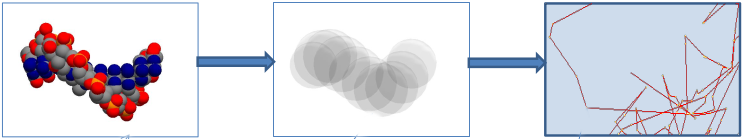
\includegraphics[width=.8\linewidth]{./Figures/aalgo.png}
    \caption[Caja delimitadora]{Caja delimitadora, lista de esferas, deposición de energía, imagen tomadas de \cite{handson} }
    \label{fig:deepbox}
\end{figure}

\begin{figure}[htbp]
    \centering
    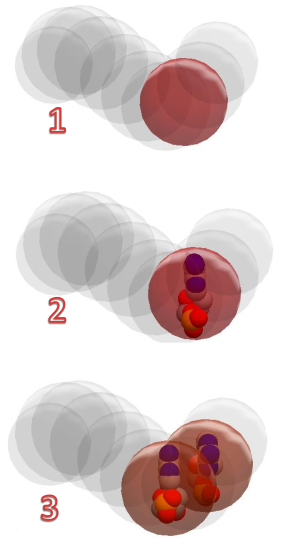
\includegraphics[width=.3\linewidth]{./Figures/algo.png}
    \caption[Esferas ligadas y nucleótidos]{Esferas ligadas y nucleótidos, imagen tomada de \cite{handson}}
    \label{fig:algoritmo}
\end{figure}

\subsubsection{Rompimientos simples y dobles}
El cálculo de rompimientos simples se hace a partir  de la asunción de que la energía sobrepase un estimado de 8.22 eV en un grupo de azúcar fosfato, es decir en un enlace fosfodiéster, para los rompimientos dobles se asume que la distancia máxima son diez pares base separando dos rompimientos simples en cadenas de ADN opuestas, cuando esto sucede se considera que ha sucedido un rompimiento doble\cite{pdblib}, esto puede ser observado en la figura ~\ref{fig:sbdb}.

\begin{figure}[htbp]
    \centering
    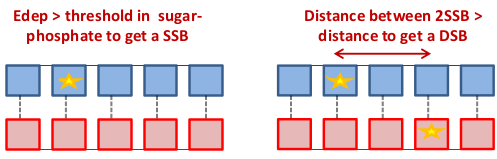
\includegraphics[width=.8\linewidth]{./Figures/romp.png}
    \caption[Esquema rompimientos simples y dobles en el ADN]{Esquema rompimientos simples y dobles en el ADN, imagen tomada de \cite{handson} }
    \label{fig:sbdb}
\end{figure}

Al principio de la simulación se crea un registro para cada cadena de ADN, los valores de dicho registro corresponden a los id de los nucleótidos y la deposición total de energía por cada evento, lo cual se tiene correlación al seguimiento de una partícula primaria y todas sus  segundarías, los registros son actualizados cada vez que el algoritmo para encontrar el átomo más cercano se completa correctamente, al final de cada evento, los registros son leídos para computar el número de rompimientos simples y dobles, cuando la simulación termina se almacena  en un histograma de ROOT la energía total de deposición en la caja de agua, y el número de rompimientos simples y dobles\cite{pdblib}, como muestra la figura ~\ref{fig:histosbdb}.

\begin{figure}[htbp]
    \centering
    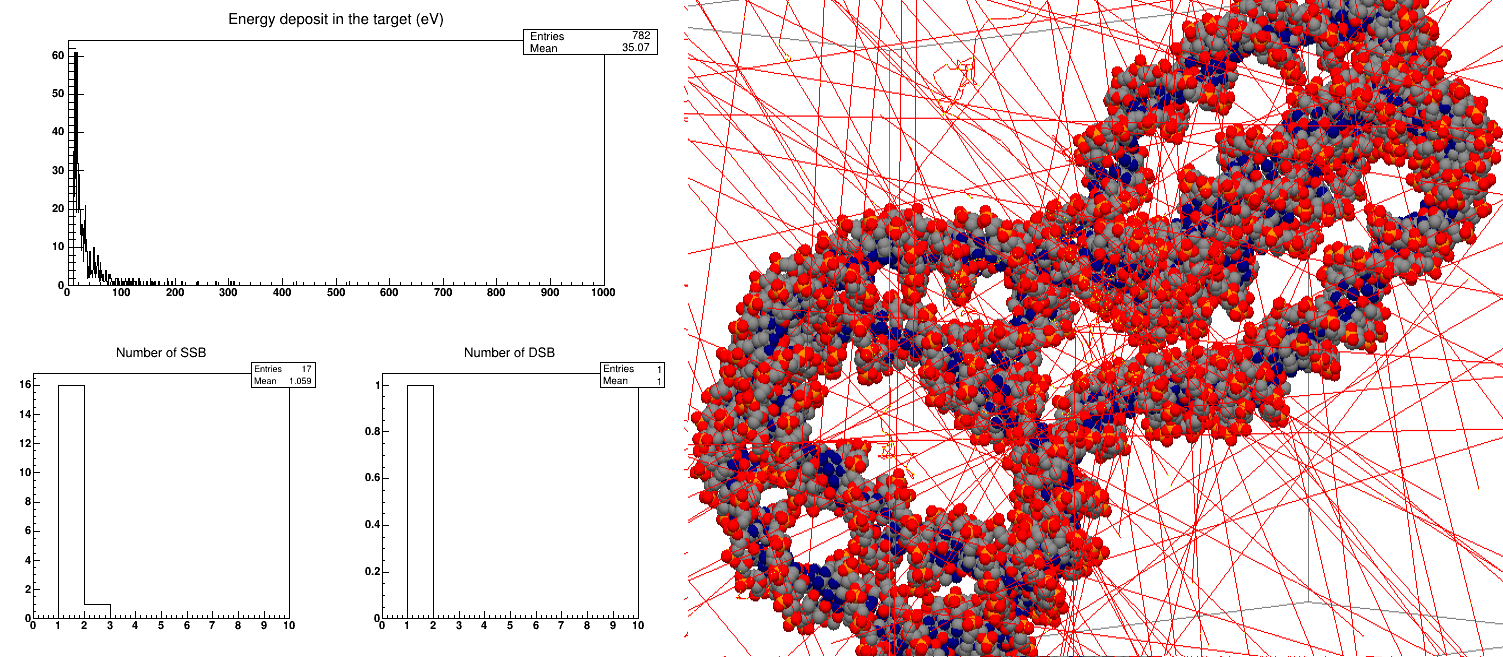
\includegraphics[width=1\linewidth]{./Figures/c1.png}
    \caption[Histograma de Root]{Histograma de Root y visualización en Geant4}
    \label{fig:histosbdb}
\end{figure}

\subsubsection{Archivos Relevantes}
Todos los ejemplos de Geant4 se componen de múltiples archivos cada uno con un propósito, esta sección aborda una explicación de los archivos fundamentales para entender pdb4dna. Un diagrama de flujo con todos los archivos de pdb4dna puede ser visto en la figura ~\ref{fig:UoC}.

\paragraph{PhysicsList}
Se encarga de llamar la física relevante para cada ejemplo, en este caso se trata de la librería "G4EmDNAPhysics" la cual contiene diversos fenómenos y procesos adaptados para nano y micro dosimetría, algunos de estos fenómenos son dispersión de Compton, dispersión de Rayleigh, efecto fotoeléctrico, etc.

\begin{figure}[htbp]
    \centering
    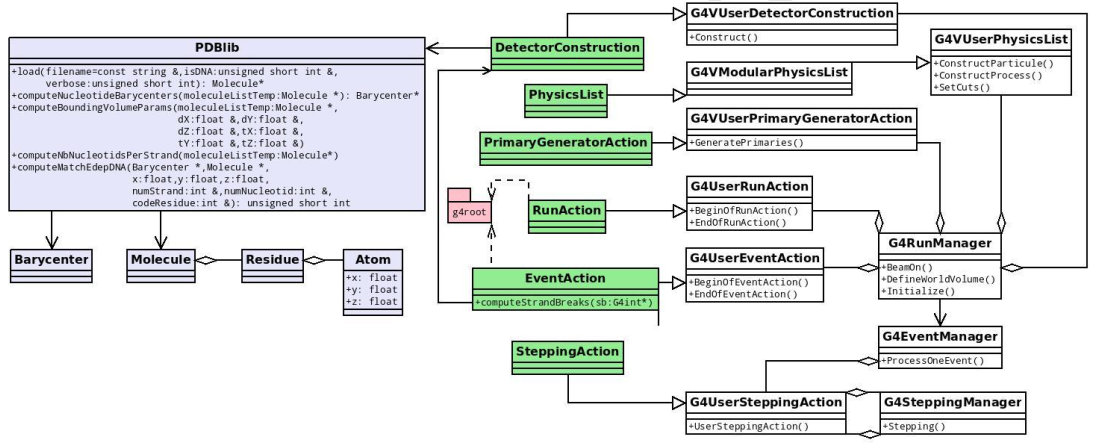
\includegraphics[width=1\linewidth]{./Figures/flujo.png}
    \caption[Diagrama de flujo de PDB4DNA]{Diagrama de flujo de PDB4DNA:Geant4 user application: Clases virtuales Geant4  (blanco), clases implementadas Geant4 (verde), librería PDB (morado) e interfaz para análisis en Root (rojo), imagen tomada de \cite{pdblib}.}
    \label{fig:UoC}
\end{figure}

\paragraph{PDBlib}

PDBlib es básicamente el corazón de PDB4DNA, es el encargado de leer el archivo de pdb, identificar si este es ADN, luego identifica las diferentes partes de la molécula de ADN como es la base, el fosfato, y el azúcar, y como el resto del código puede identificar estos para llevar a cabo el cálculo de rompimientos simples y dobles, además de ello se encarga de crear los diferentes tipos de visualización los cuales son exportados a DetectorConstruction, contiene el algoritmo para encontrar el átomo más cercano a la deposición de energía ya mencionado anteriormente.



\paragraph{DetectorConstruction}
En Geant4 este archivo se encarga de crear y posicionar los diferentes volúmenes que sean relevantes para la simulación, en el ejemplo pdb4dna es algo curioso que DetectorConstruction funciona como un archivo más de visualización para crear diferentes representaciones de la molécula de ADN, tal como se observa en las figuras: ~\ref{fig:ba}, ~\ref{fig:cpk}, ~\ref{fig:re}, sin embargo es pertinente mencionar que igual mantiene su objetivo de controlar características relevantes para la simulación como el tamaño del mundo( volumen madre donde se encuentran otros volúmenes) y el bounding box ya mencionado anteriormente.


\paragraph{SteppingAction}
Es el encargado de seguir la deposición de energía en el bounding box, primero el PDBlib se encarga de asignar un numero en base a la estructura del ADN es decir se asignan los valores numéricos: 0 para el fosfato, 1 para el azúcar y 2 para la base, esto se realiza mediante la estructura del pdb, cuando se corre un evento SteppingAction se encarga de calcular la deposición de energía en cada uno de estos, debido a que es un enlace fosfodiéster el programa solo retorna los valores de energía depositados en el fosfato o el azúcar, estos valores son enviados a subsecuentes librerías las cuales se encargan de realizar un conteo que consiste en que si la energía sobrepasa el valor de 8.22 eV cuenta como un rompimiento simple y si en 10 pares base en la cadena opuesta se presenta otro rompimiento se toma como rompimiento doble, como se muestra en la figura ~\ref{fig:sbdb}, luego todos estos datos para múltiples eventos son enviados a un archivo Root para la visualización del histograma.
